\subsection{Heurística de Búsqueda Tabú}

En este sector, se busca resolver el problema de CMF a partir de una Heurística de Búsqueda Tabú (Tabu search\footnote{Glover, F. "Tabu Search — Part I", ORSA Journal on Computing 1989}). Dicha heurística consiste en una estrategia para resolver problemas combinatorios, aplicable tanto en grafos como en otras estructuras utilizadas para resolver problemas de lógica. Este método utiliza el mismo procedimiento que Búsqueda Local\footnote{Ver sección anterior.} para acercarse progresivamente a una mejor solución dentro de un entorno. Dado que en ciertos casos la solución no puede ser mejorada, la técnica de Búsqueda Tabú permite empeorarla parcialmente para proseguir la búsqueda de una mejor. A su vez, esta heurística concede una estructura llamada $lista\ tabu$ con distintas utilidades. Principalmente, sirve para guardar movimientos de modo a no repetirlos y/o guardar características o soluciones, entre otras. A continuación, se encuentra explicitado el pseudocódigo\footnote{http://www.dc.uba.ar/materias/aed3/2013/2c/laboratorio/heuristicas.pdf} de la heurística de Búsqueda Tabú:

\begin{algorithm}[H]
\SetAlgoLined
s$_{0}$ $\leftarrow$ solucion inicial \\
s$^{*}$ $\leftarrow$ s$_{0}$ \\
T $\leftarrow$ lista tabu inicial \\
\While{ no se alcance el criterio de terminacion}{
N $\leftarrow$ vecinos de s no tabu o mejores que s$^{*}$ \\
s $\leftarrow$ mejor solucion en N. \\
\If{ s es mejor que s$^{*}$}
 {s$^{*}$ $\leftarrow$ s} 
Actualizar la lista tabu T }
\end{algorithm}

\subsubsection{Explicación del algoritmo realizado}

 El algoritmo realizado parte de un valor entero positivo ingresado como parámetro, $desviacion\_permitida$, y de una solución provista por la Heurística de Búsqueda Local. A partir de esta última, el algoritmo busca, paulatinamente, una mejor solución siguiendo las siguientes opciones:
\begin{itemize}
 \item Agregando un nodo: Dada la solución actual (una clique), procede a $agregar$ un nodo que la mejore, es decir, que aumente su frontera.
 \item Quitando un nodo: Dada la solución actual (una clique), procede a $quitar$ un nodo que la mejore, es decir, que aumente su frontera.
\end{itemize}
A diferencia de la Búsqueda Local, se buscan nuevas soluciones que no necesariamente mejoren la solución obtenida hasta el momento pero que sí lo hagan a largo plazo. Sin embargo, dentro de las formas de empeorar la solucion, se toma aquella que empeora lo menos posible. A su vez, a medida que agregamos o quitamos un nodo lo vamos poniendo en la lista tabu. Esto lo hace sin olvidar que siempre que pueda subir lo va a hacer, entonces, si descendiendo se encuentra con que puede volver a ascender, lo va a hacer hasta volver a estar en un máximo local.\newline

\begin{figure}[H] %[h] Aqui [b] para button [t] para top
\begin{center}
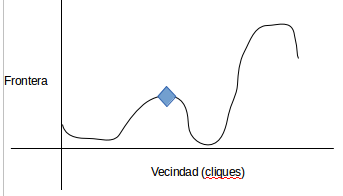
\includegraphics[width=250pt]{../imgs/1_tabu.png}
\caption{Ejemplo}
\end{center}
\end{figure}


\begin{figure}[H] %[h] Aqui [b] para button [t] para top
\begin{center}
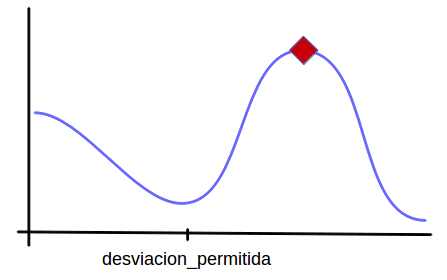
\includegraphics[width=250pt]{../imgs/2_tabu.png}
\caption{Ejemplo}
\end{center}
\end{figure}

Al finalizar, el algoritmo retorna la mejor solución hallada. \newline

\textbf{Descripcion de la lista tabu} \newline

 A medida que se van agregando o quitando nodos que no mejoran la solucion estos nodos se van marcando como tabu. De esta forma se le asigna una prioridad a cada nodo que depende de cuando fue agregado. A su vez, sea cual sea la prioridad del ultimo agregado, no se puede utilizar en la iteracion siguiente, esto es para evitar ciclar soluciones. Esto lo logramos haciendo que en el peor de los casos solo se puedan usar los nodos tabus que tienen prioridad menor a la mitad de la prioridad maxima. \newline

\textbf{Criterio de terminacion} \newline

 La terminacion de este algoritmo va a estar dada por dos factores, por un lado, la cantidad de iteraciones en que la solucion puede mejorar, y por otro, por la variable $desviacion\_permitida$ ingresada como parametro. El primero es seguro que es acotado ya que el maximo absoluto esta dado por la solucion exacta del problema, entonces, puede haber muchos maximos locales pero ninguno va a superar el maximo absoluto (esto es trivial). Por otro lado, la variable $desviacion\_permitida$ va disminuyendo cada vez que modifico la solucion actual sin mejorarla, es decir, que permitimos avanzar de manera "no creciente" una cantidad $desviacion\_permitida$ de veces. \newline


\begin{algorithm}[H]
    \SetAlgoLined
    \caption{TabuSearch}
    \KwIn{\textbf{Conj(nodos)} $solución\_inicial$, \textbf{Grafo} $g$, \textbf{Entero} $desviacion\_permitida$}
    \KwOut{\textbf{Conj(nodos)} $solución\_final$}

	\textbf{Conj(nodos)} sol$_{0}$,sol$_{1}$ \\ 
	\textbf{Conj(nodos)} $solución\_actual$ $\leftarrow$ LocalSearch($solución\_inicial$, $g$)	\\	
	\textbf{Conj(nodos)} $solución\_final$ $\leftarrow$ $solución\_actual$	\\	
	\textbf{Lista Tabu} $\leftarrow$ $\{\}$\\
	\textbf{Boolean} $Mejore\ la\ frontera$ $\leftarrow$ true

	\While{ $Mejore\ la\ frontera$ $\vee$ 0 $<$ $desviacion\_permitida$}{

	 	sol$_{0}$ $\leftarrow$ Dame Mejor solucion agregando nodo No Tabu ($solución\_inicial$,$solución\_final$) \\
		sol$_{1}$ $\leftarrow$ Dame Mejor solucion quitando nodo No Tabu ($solución\_inicial$,$solución\_final$) \\
		\If{ frontera(sol$_{0}$) $<$ frontera(sol$_{1}$)}
			{sol$_{0}$ $\leftarrow$ sol$_{1}$}
		\eIf{ frontera($solución\_actual$) $<$ frontera(sol$_{1}$)}
			{$solución\_actual$ $\leftarrow$ sol$_{0}$ \\
			$Mejore\ la\ frontera$ $\leftarrow$ true
			}
			{$Mejore\ la\ frontera$ $\leftarrow$ false \\
			 Poner Tabu Nodo utilizado en sol$_{0}$ \\
			 $desviacion\_permitida$ - 1}
		$solución\_actual$ $\leftarrow$ sol$_{0}$ \\
		\If{ frontera($solución\_final$) $<$ frontera($solución\_actual$) } 
		{$solución\_final$ $\leftarrow$ $solución\_actual$}			
	}

    	\textbf{devolver} $solución\_final$ \\

\end{algorithm}

\begin{algorithm}[H]
    \SetAlgoLined
    \caption{Dame Mejor solucion agregando nodo No Tabu}

	$solución\_final$ $\leftarrow$ $solución\_inicial$ sin un nodo cualquiera \\
	\ForAll{$u \in Candidatos\_clique($solución\_inicial$)$}{
	 		\If{$u$ $\notin Nodos(solución\_inicial)$}{
				\eIf{$\neg$ es tabu($u$)}{
		 			\If{frontera($solución\_final$) $<$ frontera( $solución\_inicial$ con $u$) }{
						$solución\_final$ $\leftarrow$ $solución\_inicial$ con $u$}
				}{
					\If{ Es Tabu aceptable ($u$) $\land$ frontera($solución\_final$) $<$ frontera( $solución\_inicial$ con $u$)}
					{$solución\_final$ $\leftarrow$ $solución\_inicial$ con $u$}
				
				}
			}
	}

\end{algorithm}

\begin{algorithm}[H]
    \SetAlgoLined
    \caption{Dame Mejor solucion quitando nodo No Tabu}

	$solución\_final$ $\leftarrow$ $solución\_inicial$ sin un nodo cualquiera \\
	\ForAll{$u \in$ Nodos($solución$\_$inicial$)}{
		\eIf{$\neg$ es tabu($u$)}{
	 		\If{frontera($solución\_final$) $<$ frontera( $solución\_inicial$ sin $u$)}{
	 			$solución\_final$ $\leftarrow$ $solución\_inicial$ sin $u$}
		}{
				\If{Es Tabu aceptable ($u$) $\land$ frontera($solución\_final$) $<$ frontera($solución\_inicial$ con $u$)}
					{$solución\_final$ $\leftarrow$ $solución\_inicial$ con $u$}
		}
	}

\end{algorithm}

Donde:
\begin{itemize}
 \item $desviacion$\_$permitida$ Dice la cantidad de veces que se agrega o quita un nodo por iteracion (empeorando la solución parcial).
 \item frontera : Dice, dada una solución como parametro, el numero de nodos adyacentes a la frontera (es lo que pide maximizar el enunciado).
 \item Candidatos$\_$clique : Dice los nodos que pertenecen a la clique maxima de los nodos pasados como parametro.
 \item Nodos : Da los nodos pertenecientes a la solución pasada como parametro.
 \item Es Tabu aceptable : Un nodo perteneciente a la lista tabu es aceptable si su prioridad es menor a la mitad de la prioridad maxima.
\end{itemize}

\subsubsection{Complejidad Temporal}
\subsubsection{Instancias problemáticas}
\subsubsection{Experimentación}
